\section{PDF space estimators}

We can calculate the same set of estimators in PDF space with minor alteration
to the definitons. Firstly, we are free to choose our own data points which will
be points in x and flavour for the PDFs at the initial scale. For this study the
points in x for singlet and gluon were chosen to be half logarithmically spaced
between $10^-3<x<0.1$ and half linearly spaced between $0.1<x<0.5$. For the
other flavours (V, V3, V8, T3, and T8) we simply choose the points to be
linearly spaced $0.1<x<0.5$ which is supposed to roughly capture the data
region of the PDFs.

The covariance matrix which is used in the definition
of bias and variance is estimated from the union of all of the replicas, allowing
for correlations across different flavours. We can also calculate $\xi_{1\sigma}$
in the basis which diagonalises this covariance matrix and show that this gives
much good agreement between the expected $\xi_{1\sigma}$ and that measured
directly from the PDFs.

\subsection{Stability of estimated covariance matrix}

Before looking at the estimators, it's useful to see how stable the covariance
matrix estimated from the PDF replicas is under variations of the number of x
points for each flavour. We show the eigenvalues of the correlation matrices
for $N_x = 4,\,6$ and $12$. We see that the l2-condition number of the
correlation matrix starts to increase with $N_x$ rapidly even between $N_x=4$
and $N_x=6$. This leads us to conclude that bias, variance and $\xi_{1\sigma}$
in the basis which diagonalises the covariance matrix might have reliability
issues beyond $N_x = 4$ because the amount of statistics to accurately
calculate the covariance matrix becomes much greater.

\begin{figure}[]
    \centering
    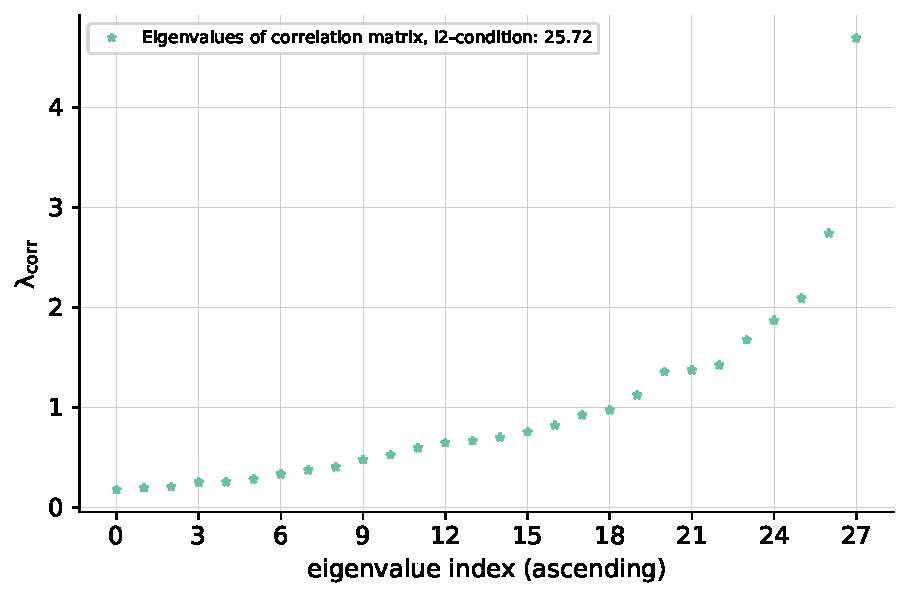
\includegraphics[width=0.8\textwidth]{corr_eval_nx4.pdf}
    \caption{The eigenvalues of the correlation matrix for the total correlation
    matrix, for all flavours and x, with $N_x=4$. The matrix is estimated from
    30 fits, each with 40 replicas.
    The l2-condition number, 25.72, is the ratio of the
    largest eigenvalue over the smallest. We see that all the eigenvalues are
    fairly similar order of magnitude, which means the points are not too correlated
    and we would expect a better estimate of the correlations with a smaller
    number of replicas.}
    \label{fig:correignx4}
\end{figure}

\begin{figure}[]
    \centering
    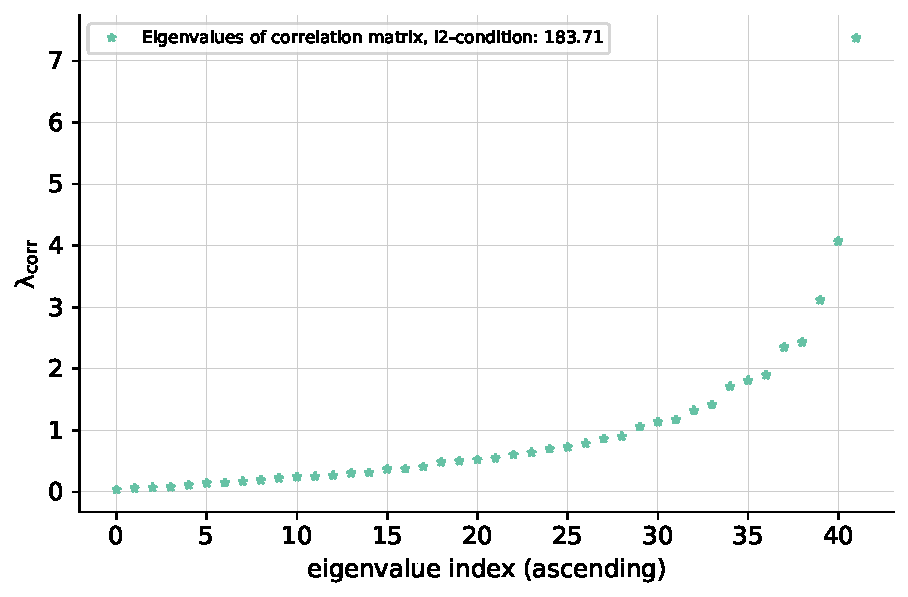
\includegraphics[width=0.8\textwidth]{corr_eval_nx6.pdf}
    \caption{The eigenvalues of the correlation matrix for the total correlation
    matrix, for all flavours and x, with $N_x=6$. The matrix is estimated from
    30 fits, each with 40 replicas.
    The l2-condition number, 183.71, is the ratio of the
    largest eigenvalue over the smallest. The condition number is already markedly
    bigger than in figure \ref{fig:correignx4} and so we might expect that
    our estimate from 1200 total replicas is already deteriorating in reliability.}
    \label{fig:correignx6}
\end{figure}

\begin{figure}[]
    \centering
    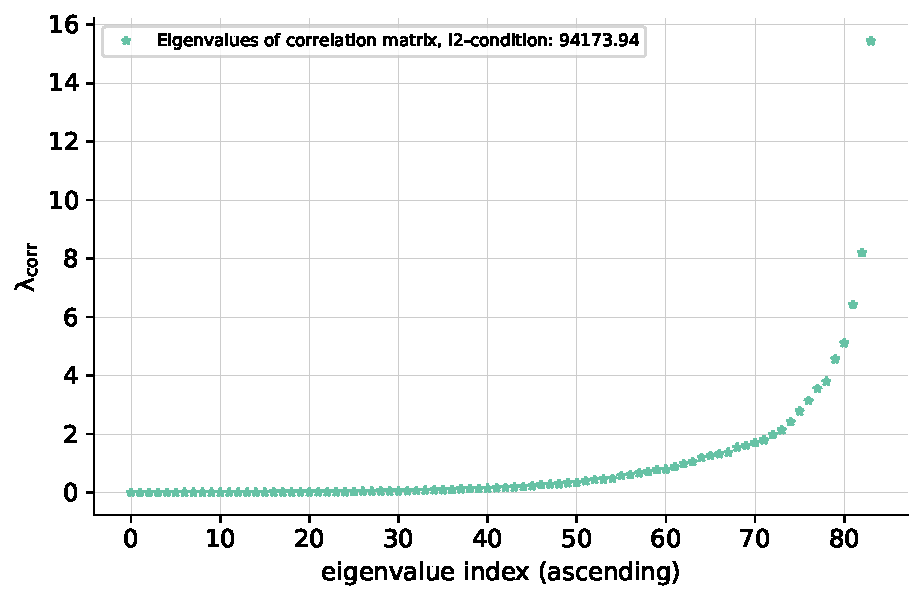
\includegraphics[width=0.8\textwidth]{corr_eval_nx12.pdf}
    \caption{The eigenvalues of the correlation matrix for the total correlation
    matrix, for all flavours and x, with $N_x=12$. The matrix is estimated from
    30 fits, each with 40 replicas.
    The l2-condition number, 94173.94, is the ratio of the
    largest eigenvalue over the smallest. The condition number is considerably
    greater than for $N_x=4$ and so the estimate of the correlations is likely
    very unreliable.}
    \label{fig:correignx12}
\end{figure}

\subsection{Results for $N_x=4$}

Given the eigenvalue plots in the previous section we first look at estimators
which rely on estimation of a covariance matrix for $N_x=4$. This should ensure
more reliable results. The two estimators considered here are
$\sqrt{\frac{\eshift{\bias}}{\eshift{\var}}}$ and $\xi_{1\sigma}$ in the basis
which diagonalises the estimated covariance matrix. First a table of
$\sqrt{\frac{\eshift{\bias}}{\eshift{\var}}}$ for each flavour, and the total
which allows for correlations between flavours. The table has two columns
for the mean and standard deviation across 100 bootstrap samples.

\begin{tabular}{lrr}
\toprule
{} &  bootstrap mean sqrt ratio &  bootstrap std. sqrt ratio \\
flavour  &                            &                            \\
\midrule
\$\textbackslash Sigma\$ &                       0.90 &                       0.05 \\
gluon    &                       0.90 &                       0.05 \\
V        &                       1.02 &                       0.06 \\
V3       &                       0.99 &                       0.05 \\
V8       &                       0.91 &                       0.06 \\
T3       &                       0.62 &                       0.03 \\
T8       &                       1.31 &                       0.05 \\
Total    &                       0.92 &                       0.03 \\
\bottomrule
\end{tabular}


Now a table for $\xi_{1\sigma}$ in the diagonal basis, with two columns, with the
mean and std. dev. across 100 bootstrap samples.

\begin{tabular}{lrr}
\toprule
{} &  bootstrap mean \$\textbackslash xi\_\{1\textbackslash sigma\}\$ &  bootstrap std. \$\textbackslash xi\_\{1\textbackslash sigma\}\$ \\
flavour  &                                 &                                 \\
\midrule
\$\textbackslash Sigma\$ &                            0.70 &                            0.04 \\
gluon    &                            0.69 &                            0.03 \\
V        &                            0.66 &                            0.05 \\
V3       &                            0.63 &                            0.04 \\
V8       &                            0.71 &                            0.04 \\
T3       &                            0.89 &                            0.03 \\
T8       &                            0.46 &                            0.04 \\
Total    &                            0.71 &                            0.02 \\
\bottomrule
\end{tabular}


As with the estimators in data-space we can compare the expected $\xi_{1\sigma}$
from $\sqrt{\frac{\eshift{\bias}}{\eshift{\var}}}$ by using eq. \eqref{eq:expectedxi}
to the measured $\xi_{1\sigma}$.

\begin{center}
    \resizebox{0.6\textwidth}{!}{\begin{tabular}{lrr}
        \toprule
        {} &  Measured $\xi_{\sigma}$ &  Expected $\xi_{\sigma}$ from bias/variance \\
        flavour  &                           &                           \\
        \midrule
        $\Sigma$ &                      0.73 &                      0.75 \\
        gluon    &                      0.68 &                      0.75 \\
        V        &                      0.70 &                      0.69 \\
        V3       &                      0.63 &                      0.70 \\
        V8       &                      0.73 &                      0.74 \\
        T3       &                      0.92 &                      0.91 \\
        T8       &                      0.43 &                      0.57 \\
        Total    &                      0.72 &                      0.75 \\
        \bottomrule
        \end{tabular}}
\end{center}

We see very good agreement between the two estimators. Also, the numbers
are very comparable to those calculated in the space of data, for data not
included in the fit.

\subsection{Results in x-basis}

Alternatively we can try calculating $\xi_{1\sigma}$ in the x-basis and ignore
any correlations. This still will give an indication of whether the distribution
at each point in x is similar between the PDF replicas for a given fit and the 
expectation of the PDF replicas at each point in x across fits. Since there
is no covariance matrix calculation we are free to increase the number of points
in x, with the caveat that the average of $\xi_{1\sigma}^i$ across x values
becomes the average of an increasingly correlated sample of points.

First the values of $\xi_{1\sigma}$ in the x-basis for $N_x=4$

\begin{center}
    \resizebox{0.6\textwidth}{!}{\begin{tabular}{lrr}
        \toprule
        {} &  bootstrap mean $\xi_{1\sigma}$ &  bootstrap std. dev.  $\xi_{1\sigma}$ \\
        flavour  &                                 &                                 \\
        \midrule
        $\Sigma$ &                            0.77 &                            0.04 \\
        gluon    &                            0.65 &                            0.04 \\
        V        &                            0.63 &                            0.05 \\
        V3       &                            0.69 &                            0.04 \\
        V8       &                            0.71 &                            0.04 \\
        T3       &                            0.88 &                            0.03 \\
        T8       &                            0.39 &                            0.03 \\
        Total    &                            0.67 &                            0.02 \\
        \bottomrule
        \end{tabular}}
\end{center}

and the same table except for $N_x=12$

\begin{center}
    \resizebox{0.6\textwidth}{!}{\begin{tabular}{lrr}
        \toprule
        {} &  bootstrap mean $\xi_{1\sigma}$ &  bootstrap std. dev. $\xi_{1\sigma}$ \\
        flavour  &                                 &                                 \\
        \midrule
        $\Sigma$ &                            0.74 &                            0.04 \\
        gluon    &                            0.57 &                            0.03 \\
        V        &                            0.65 &                            0.05 \\
        V3       &                            0.71 &                            0.03 \\
        V8       &                            0.76 &                            0.04 \\
        T3       &                            0.88 &                            0.03 \\
        T8       &                            0.38 &                            0.03 \\
        Total    &                            0.67 &                            0.02 \\
        \bottomrule
        \end{tabular}}
\end{center}

Something
which is quite reassuring is that the $\xi_{1\sigma}$ is stable under variations
of $N_x$.

Finally we can plot $\xi_{1\sigma}$ for each point in x. Here the plots were
produced with $N_x=4$, for which we can reliably look at results in both the
x-basis and the basis which diagonalises the covariance matrix estimated
from the replicas

\begin{figure}
    \centering
    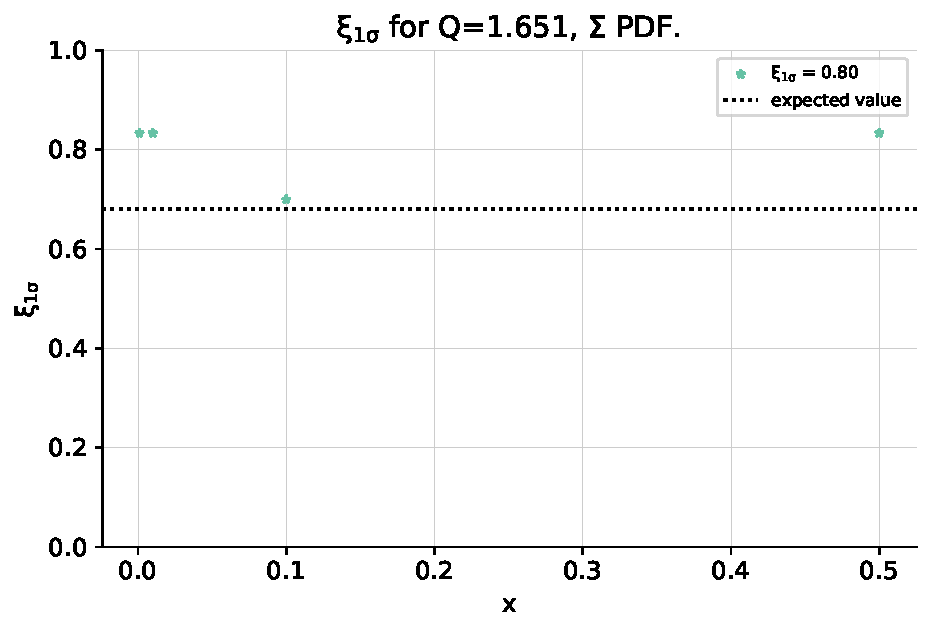
\includegraphics[width=0.6 \textwidth]{plot_xi_xbasis_sigma.pdf}
    \caption{
        $\xi^{i}_{1\sigma}$ for singlet PDF, in the x-basis, $N_x=4$. Note that
        the first two points are logarithmically spaced from $10^{-3} < x < 0.1$
        and the second two points are linearly spaced between $0.1 < x < 0.5$.}
    \label{fig:pdfxisinglet}
\end{figure}

\begin{figure}
    \centering
    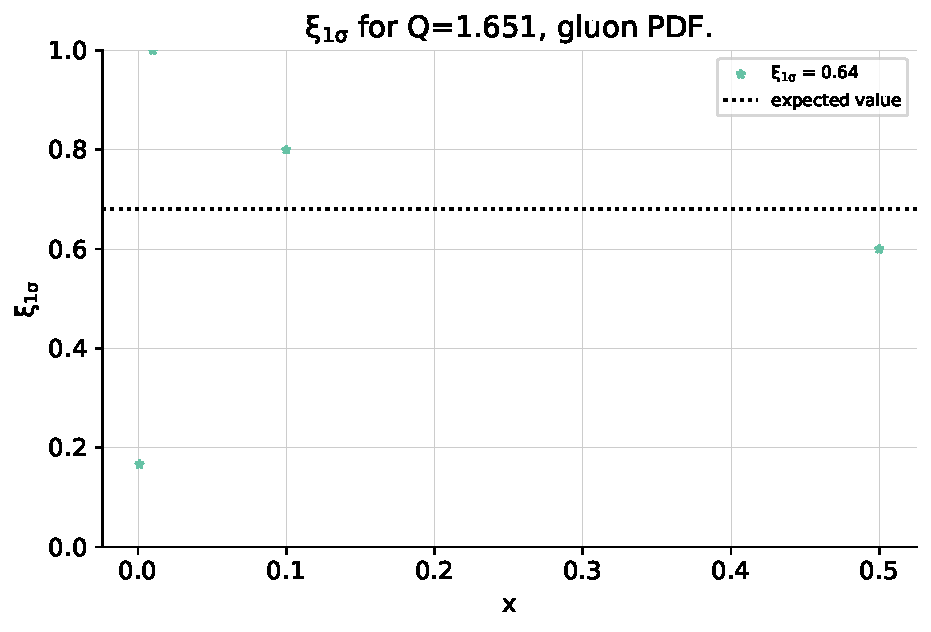
\includegraphics[width=0.6 \textwidth]{plot_xi_xbasis_gluon.pdf}
    \caption{
        $\xi^{i}_{1\sigma}$ for gluon PDF, in the x-basis, $N_x=4$. Note that
        the first two points are logarithmically spaced from $10^-3 < x < 0.1$
        and the second two points are linearly spaced between $0.1 < x < 0.5$.
    }
    \label{fig:pdfxigluon}
\end{figure}

\begin{figure}
    \centering
    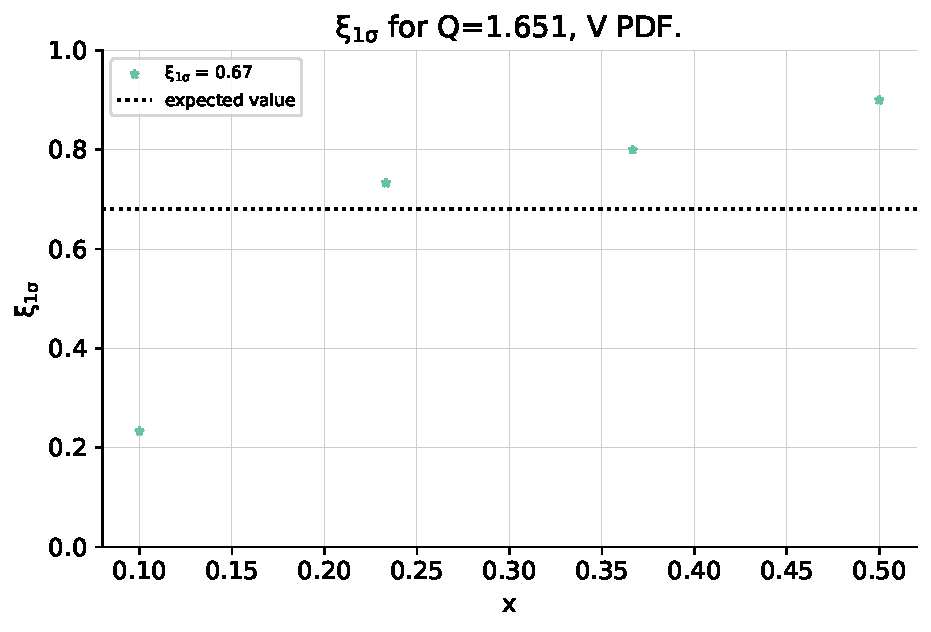
\includegraphics[width=0.6 \textwidth]{plot_xi_xbasis_v.pdf}
    \caption{
        $\xi^{i}_{1\sigma}$ for V PDF, in the x-basis, $N_x=4$. Note that
        the first two points are logarithmically spaced from $10^-3 < x < 0.1$
        and the second two points are linearly spaced between $0.1 < x < 0.5$.
    }
    \label{fig:pdfxiv}
\end{figure}

\begin{figure}
    \centering
    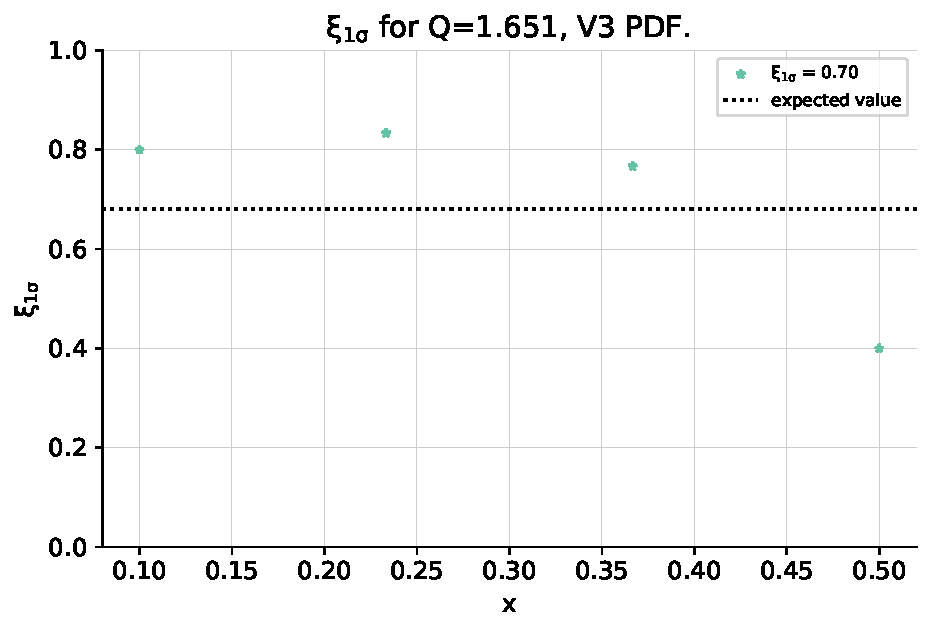
\includegraphics[width=0.6 \textwidth]{plot_xi_xbasis_v3.pdf}
    \caption{
        $\xi^{i}_{1\sigma}$ for V3 PDF, in the x-basis, $N_x=4$. Note that
        the first two points are logarithmically spaced from $10^-3 < x < 0.1$
        and the second two points are linearly spaced between $0.1 < x < 0.5$.
    }
    \label{fig:pdfxiv3}
\end{figure}

\begin{figure}
    \centering
    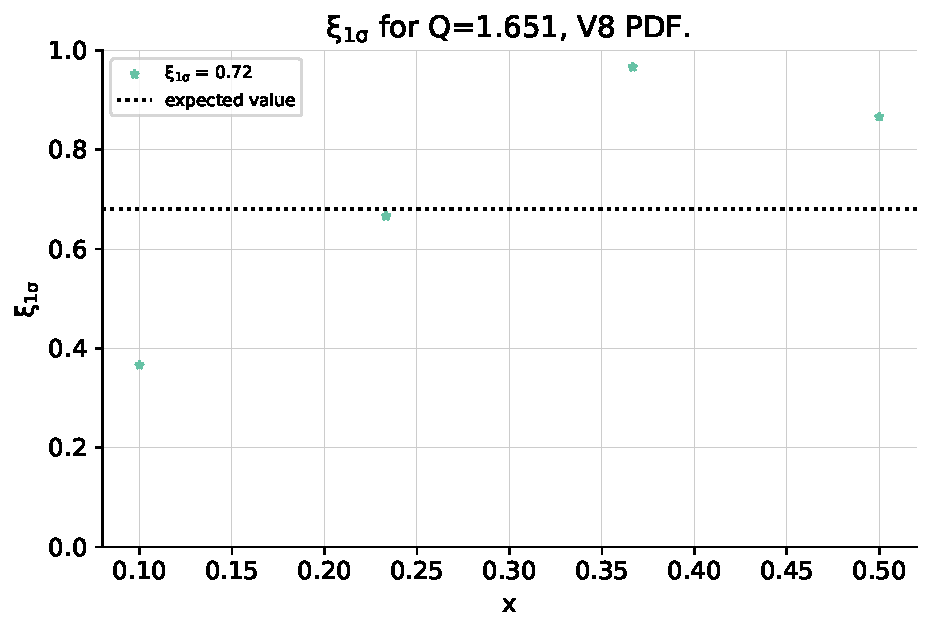
\includegraphics[width=0.6 \textwidth]{plot_xi_xbasis_v8.pdf}
    \caption{
        $\xi^{i}_{1\sigma}$ for V8 PDF, in the x-basis, $N_x=4$. Note that
        the first two points are logarithmically spaced from $10^-3 < x < 0.1$
        and the second two points are linearly spaced between $0.1 < x < 0.5$.
    }
    \label{fig:pdfxiv8}
\end{figure}

\begin{figure}
    \centering
    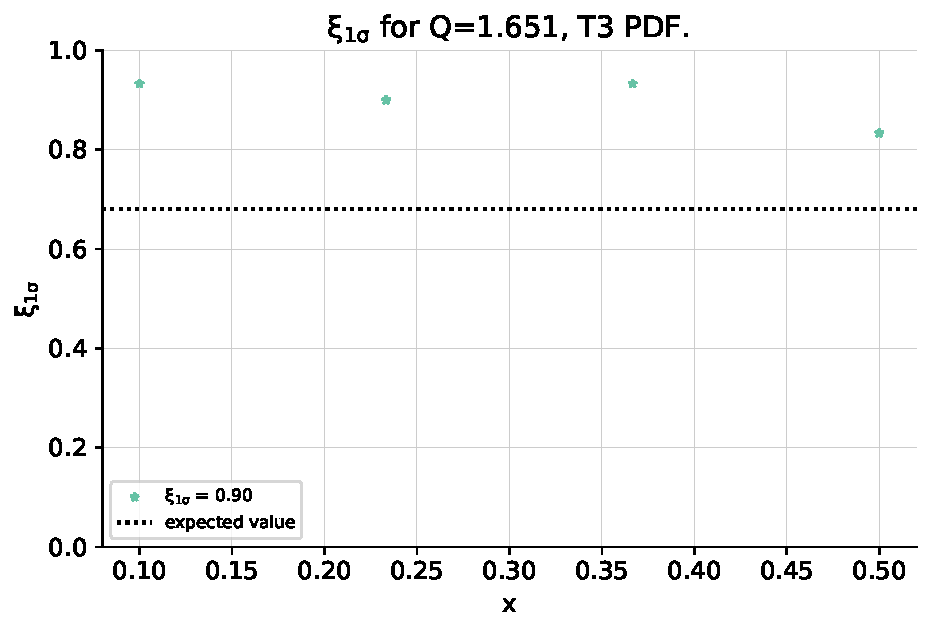
\includegraphics[width=0.6 \textwidth]{plot_xi_xbasis_t3.pdf}
    \caption{
        $\xi^{i}_{1\sigma}$ for T3 PDF, in the x-basis, $N_x=4$. Note that
        the first two points are logarithmically spaced from $10^-3 < x < 0.1$
        and the second two points are linearly spaced between $0.1 < x < 0.5$.
    }
    \label{fig:pdfxit3}
\end{figure}

\begin{figure}
    \centering
    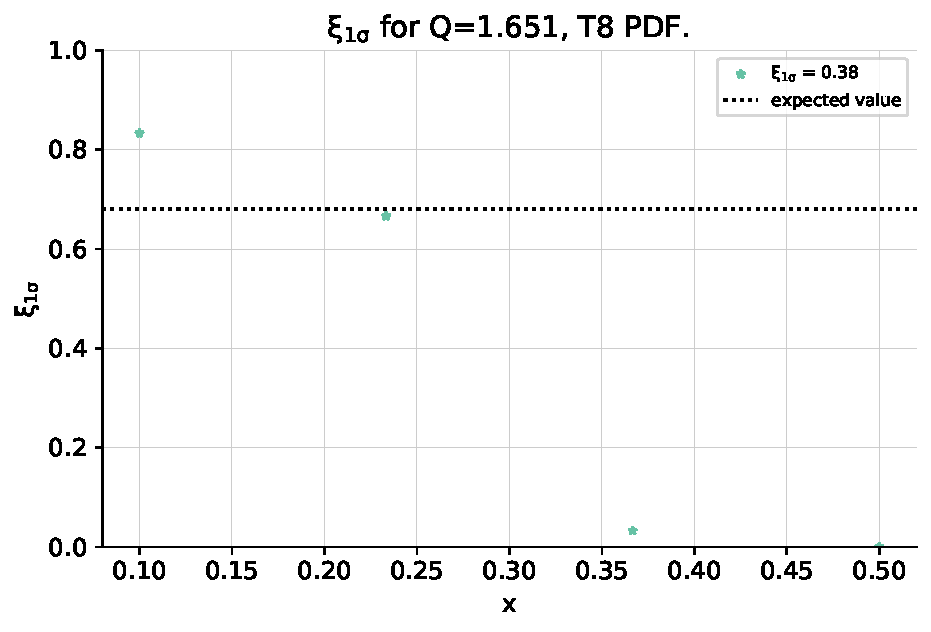
\includegraphics[width=0.6 \textwidth]{plot_xi_xbasis_t8.pdf}
    \caption{
        $\xi^{i}_{1\sigma}$ for T8 PDF, in the x-basis, $N_x=4$. Note that
        the first two points are logarithmically spaced from $10^-3 < x < 0.1$
        and the second two points are linearly spaced between $0.1 < x < 0.5$.
    }
    \label{fig:pdfxit8}
\end{figure}

\subsection{Summary}

The reliability of the covariance/correlation matrix is highly dependent on
$N_x$. For the number of replicas we have access to, we appear to only get a
reasonable result for $N_x=4$. For that value of $N_x$ we see good agreement
between $\sqrt{\frac{\eshift{\bias}}{\eshift{\var}}}$ and $\xi_{1\sigma}$.

We can also look at $\xi_{1\sigma}$ in the x-basis. We see that results are
much more stable under varying $N_x$ despite the fact that we are neglecting
correlations. $\xi_{1\sigma}$ in the x-basis agrees fairly well, with boostrap
error to that calculated in the diagonal basis with $N_x=4$. We can also
plot $\xi_{1\sigma}^i$ in the x-basis and potentially use this as a diagnostic
tool to see where in x uncertainties are over/under estimated.

Generally the results for low $N_x$ or those calculated in the x-basis look good
and seem consistent with the results for data which was not included in the fit.
